\documentclass{ohm_project_description}

\projecttitle{Drone Light Painting – Koordinierte Lichtbilderzeugung mit Micro-Drohnen}
\projectauthor{Labor für mobile Robotik}
\projectdate{2026}

\begin{document}

\maketitle
\thispagestyle{fancy}

\vspace*{-2.5cm}
\begin{figure}[h!]
    \centering
    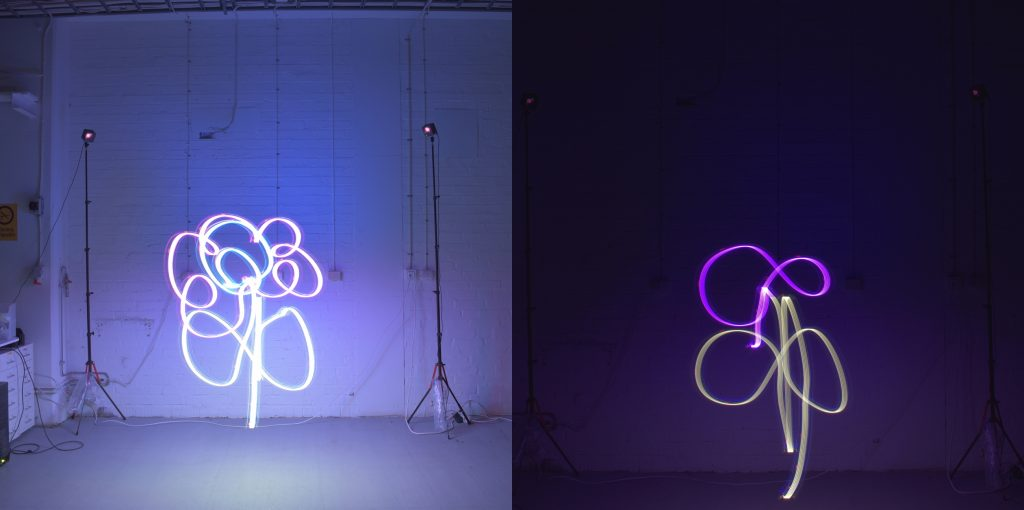
\includegraphics[height=4cm]{img/lightpainting.png}
\end{figure}

Seit kurzem steht am AerodrOHM eine Gruppe kleiner Micro-Drohnen (Crazyflies) zur Verfügung, die für koordinierte Formationsflüge programmiert werden können. Ziel dieser Arbeit ist die Umsetzung einer Demonstration im Stil von Drone Light Painting: Die Drohnen führen vordefinierte Flugmuster aus und erzeugen dadurch räumliche Lichtbilder, die per Langzeitbelichtung fotografisch festgehalten werden können.

Im ersten Schritt sollen geeignete Flugbahnen entworfen werden, die sowohl einfache geometrische Formen als auch komplexere Muster wie Schriftzüge oder Logos umfassen können. Die Trajektorien müssen so geplant werden, dass Kollisionen zwischen den Drohnen zuverlässig vermieden werden und die zeitliche Synchronisation der Flugbewegungen sichergestellt ist. Aufbauend auf der Trajektorienplanung soll die koordinierte Ansteuerung mehrerer Drohnen im Schwarm realisiert werden. Die praktische Erprobung findet im Flugraum des AerodrOHM statt.

\section*{Arbeitspakete}
\begin{itemize}[leftmargin=0.5cm]
    \setlength\itemsep{.1em}
    \item Einarbeitung in die Drohnenplattform und die Programmierschnittstelle
    \item Entwurf und Implementierung von Flugbahnen für verschiedene Lichtmuster
    \item Koordination und Synchronisation mehrerer Drohnen im Schwarm
    \item Experimentelle Erprobung und fotografische Dokumentation der Lichtbilder
\end{itemize}

\section*{Voraussetzungen}
\begin{itemize}[leftmargin=0.5cm]
    \setlength\itemsep{.1em}
    \item Gute Programmierkenntnisse in Python
    \item Interesse an autonomem Flug und Mehrrobotersystemen
    \item Grundlegendes Verständnis von Koordinatensystemen und räumlicher Geometrie
\end{itemize}

\vspace{0.5cm}
Das Thema kann nach Abstimmung als \textbf{Projekt-, Bachelor- oder Masterarbeit} bearbeitet werden.

\vfill
\textcolor{ohm_red}{\rule{\linewidth}{0.4mm}}
\textbf{\textcolor{ohm_red}{Labor für mobile Robotik}} \\
\begin{tabular}{@{}ll}
\textbf{Betreuer:} & Prof. Dr. Christian Pfitzner \\
\textbf{E-Mail:}   & \href{mailto:christian.pfitzner@th-nuernberg.de}{christian.pfitzner@th-nuernberg.de} \\
\end{tabular}

\end{document}
